%% abtex2-modelo-include-comandos.tex, v-1.9.6 laurocesar
%% Copyright 2012-2016 by abnTeX2 group at http://www.abntex.net.br/ 
%%
%% This work may be distributed and/or modified under the
%% conditions of the LaTeX Project Public License, either version 1.3
%% of this license or (at your option) any later version.
%% The latest version of this license is in
%%   http://www.latex-project.org/lppl.txt
%% and version 1.3 or later is part of all distributions of LaTeX
%% version 2005/12/01 or later.
%%
%% This work has the LPPL maintenance status `maintained'.
%% 
%% The Current Maintainer of this work is the abnTeX2 team, led
%% by Lauro César Araujo. Further information are available on 
%% http://www.abntex.net.br/
%%
%% This work consists of the files abntex2-modelo-include-comandos.tex
%% and abntex2-modelo-img-marca.pdf
%%

% ---
% Este capítulo, utilizado por diferentes exemplos do abnTeX2, ilustra o uso de
% comandos do abnTeX2 e de LaTeX.
% ---

\chapter{Métodos Computacionais}

\section{A função de onda na mecânica quântica}
	
	Desde o clássico experimento de dupla fenda feito por Thomas Young no início do século XIX e os trabalhos de Max Planck sobre a quantização da luz \cite{planck1914warmestrahlung}, é um fato notadamente aceito que os fótons apresentam um caráter dual, possuindo propriedades tanto de partícula quanto de onda (propriedade conhecida na literatura como \textit{dualidade partícula-onda}). Com o intuito de descrever o caráter de partícula da luz, Einstein, em 1905 \cite{einstein1905heuristic}, propôs expressar a energia $E$ e o momento $p$ de um fóton como:
	\begin{equation}
		E = h\nu = \hbar \omega ; \quad p = \frac{E}{c} = \frac{h}{\lambda} = \hbar k
	\end{equation}
	
	onde $\nu$ é a frequência do fóton, $\omega = 2\pi \nu$ é a frequência angular, $\lambda$ é o comprimento de onda do fóton, $k=|\textbf{k}| = 2\pi/\lambda$ é o número de onda ($\textbf{k}$ é o vetor de onda) e $\hbar = h/2\pi$ é a constante de Plank reduzida. 
	
	Em 1923, de Broglie propôs que toda a matéria, não somente os fótons, possuem uma natureza ondulatória. Para uma partícula material livre, de Broglie assumiu que a onda associada a essa partícula também possui uma frequência $\nu_d$ e um comprimento de onda $\lambda_d$ \cite{broglie1923waves}: 
	
	\begin{equation} 
		\nu_d = \frac{E}{h}, \quad \lambda_d = \frac{h}{p}
		\label{einstein}
	\end{equation}
	
	Desconsiderando efeitos relativísticos, o comprimento de onda de de Broglie de uma partícula de massa $m$ e velocidade $v$ pode ser obtida diretamente:
	
	\begin{equation}
		\lambda_d = \frac{h}{mv} = \frac{h}{\sqrt{2mE_k}}
	\end{equation}
	
	onde $E_k = mv^2/2$ é a energia cinética da partícula. 
	
	Motivado pela proposição de de Broglie, no princípio de conservação de energia e nas equações clássicas de ondas planas, em 1926 Erwin Schrödinger propôs uma equação que descreve o comportamento ondulatório da matéria. Em um campo conservativo (campo de forças central), a energia mecânica total $E$ de uma partícula material é conservada:
	
	\begin{equation}
		E_k + E_p = \frac{\textbf{p}^2}{2m} + V(\textbf{r}) = E
		\label{e_schrodinger}
	\end{equation}
	
	onde $V(\textbf{r})$ é a energia potencial e $m$ a massa da partícula. Utilizando as relações de Einstein para expressar a energia $E$ e o momento $\textbf{p}$ dadas pela \autoref{einstein} e utilizando a equação geral de uma onda plana comumente escrita na forma:
	
	\begin{equation}
		A(\textbf{r}, t) = A_0 exp\{i(\textbf{k} \cdot \textbf{r} - \omega t)\}
	\end{equation}
	
	e assumindo que o caráter ondulatório da matéria pode ser descrito por ondas planas, pode-se escrever
	
	\begin{equation}
		\varphi (\textbf{r}, t) = \varphi_0 exp \left\{ \frac{i}{\hbar} (\textbf{p} \cdot \textbf{r} - Et) \right\}
	\end{equation}
	
	E assim, multiplicando ambos os lados da \autoref{e_schrodinger} por $\varphi (\textbf{r}, t)$ obtêm-se
	
	\begin{equation}
		\left[ \frac{\textbf{p}^2}{2m} + V(\textbf{r})\right] \varphi (\textbf{r}, t) = E \varphi (\textbf{r}, t)
	\end{equation}
	
	Reescrevendo então o operador momento e o operador energia na forma:
	 
	\begin{equation}
		\textbf{p} = -i\hbar \nabla, \quad E=i\hbar \frac{\partial}{\partial t}
	\end{equation}
	
	expandindo o campo de forças central para um campo de forças geral ($V(\textbf{r}) \rightarrow U(\textbf{r}, t)$) e substituindo a onda plana $\varphi (\textbf{r}, t)$ por uma função de onda geral $\Psi(\textbf{r}, t)$ obtemos a amplamente conhecida equação de Schrödinger
	
	\begin{equation}
		\left[ -\frac{\hbar^2}{2m}\nabla^2 + U(\textbf{r}, t) \right]\Psi(\textbf{r}, t) = i\hbar \frac{\partial}{\partial t}\Psi(\textbf{r}, t)
	\end{equation}
	
	
	Na mecânica quântica, o \textbf{estado} de um sistema físico qualquer é descrito pela função de estado $\Psi = \Psi(\textbf{r}, t)$, onde a quantidade real e positiva $|\Psi(\textbf{r}, t)|^2$ é interpretada como a densidade de probabilidade de encontrar-se o sistema no ponto $\textbf{r}$, caso a medida da coordenada $\textbf{r}$ for realizada. 
	
	Existe uma forma alternativa de escrever a equação de Schrödinger, utilizando uma notação proposta por \citeauthor{dirac1981principles} - e portanto conhecida como \textit{notação de Dirac} - utiliza o \textit{bra} $\langle |$ e o \textit{ket} $| \rangle$ para representar os vetores de estado que constituem o espaço de Hilbert $\textit{H}$. Iremos então escrever a equação de Schrödinger utilizando a notação de Dirac e o formalismo de operadores, ficando com
	

	\begin{equation}
	\textbf{\^H}|\Psi(r,t)\rangle = i\hbar\frac{\partial}{\partial t} |\Psi(r,t)\rangle
	\label{schrodinger}
	\end{equation}
	
	onde $\hat{\textbf{H}}$ é o operador Hamiltoniano. Na ausência de uma perturbação externa que dependa explicitamente do tempo podemos reescrever a \autoref{schrodinger} na forma independente do tempo:
	
	\begin{equation}
	\label{schrodinger_it}
	\textbf{\^H}|\Psi(r)\rangle = E|\Psi(r)\rangle
	\end{equation}
	
	Em princípio, se resolvida corretamente a equação de Schrödinger nos permite obter a função de onda para o sistema e, consequentemente, toda informação possível sobre esse sistema. Entretanto, para sistemas ligeiramente mais complexos do que um único elétron confinado sob a ação de um potencial externo, a solução dessa equação é extremamente difícil (virtualmente impossível na maioria dos casos de interesse prático) de ser obtida. Dessa forma, para que seja aplicável na prática precisamos fazer uma série de aproximações. \cite{jensen2017introduction, kaufman1972accurate, levine2000quantum, szabo2012modern}
	
	\subsection{Aproximação Adiabática e Aproximação de Born-Oppenheimer}
	
	Para aplicarmos a equação de Schrödinger para átomos, a primeira aproximação a ser feita é considerar que o acoplamento do movimento do núcleo e dos elétrons pode ser negligenciado e esses movimentos tratados de maneira independente. Esse tratamento é conhecido como \textit{Aproximação de Born-Oppenheimer} \cite{born1927quantentheorie} , em homenagem aos cientistas que a propuseram. Essa aproximação permite que tratemos a posição relativa dos núcleos como um parâmetro da função de onda eletrônica, resultando em uma \textit{superfície de energia potencial} para o movimento dos núcleos. 
	
	Podemos escrever o operador Hamiltoniano como a soma das energias cinéticas (\textbf{T}) e potenciais (\textbf{V}) dos núcleos e elétrons:
	
	\begin{equation}
	\label{h_tot}
	\textbf{\^H$_{tot}$} = \textbf{\^T$_{n}$} + \textbf{\^T$_{e}$} + \textbf{\^V$_{n}$} + \textbf{\^V$_{ee}$} + \textbf{\^V$_{nn}$}
	\end{equation}
	
	Podemos então fazer uma transformação de coordenadas para escrever a \autoref{h_tot} em coordenadas relativas ao centro de massa do sistema. É importante ressaltar que esse tipo de operação não é uma aproximação, é somente uma troca de coordenadas do sistema. Após essa operação, o Hamiltoniano total do sistema continua sendo um Hamiltoniano exato e completo do sistema. Dessa forma, ficamos com
	
	\begin{equation}
	\label{h_tot2}
	\textbf{\^H$_{tot}$} = \textbf{\^T$_{n}$} + \textbf{\^H$_{e}$} + \textbf{\^H$_{pm}$} 
	\end{equation}
	
	onde 
	
	\begin{equation}
	\label{he}
	\textbf{\^H$_{e}$} = \textbf{\^T$_{e}$} + \textbf{\^V$_{ne}$} + \textbf{\^V$_{ee}$} + \textbf{\^V$_{nn}$} + \textbf{\^V$_{en}$}
	\end{equation}
	
	\begin{equation}
	\label{hmp}
	\textbf{\^H$_{mp}$} = -\frac{1}{2M_{tot}} \left( \sum_{i}^{N_{elec}} \nabla_i \right)^2
	\end{equation}
	
	com \textbf{\^H$_{e}$} sendo o \textit{operador Hamiltoniano eletrônico} e \textbf{\^H$_{pm}$} o Hamiltoniano de \textit{polarização de massa} (M$_{tot}$ é a massa total de todos os núcleos). Escrevendo explicitamente a equação para \textbf{\^H$_{e}$}  (em unidades atômicas), obtemos
	
	\begin{equation}
	\label{he2}
	\textbf{\^H$_{e}$} = -\frac{1}{2} \sum_{i}^{N_{elec}} \nabla_i^2 -  \sum_{i=1}^{N_{elec}} \sum_{A=1}^{M_{nuc}} \frac{Z_A}{r_{iA}} +  \sum_{i=1}^{N_{elec}}  \sum_{j>i}^{N_{elec}} \frac{1}{r_{ij}} +  \sum_{A=1}^{M_{nuc}} \sum_{B>A}^{M_{nuc}} \frac{Z_{A}Z_{B}}{R_{AB}}
	\end{equation}
	
	Se olharmos com atenção, perceberemos que \textbf{\^H$_{e}$} depende das posições dos núcleos (R$_A$, R$_B$ e R$_{AB}$), mas não de seus momentos. Dessa forma, o Hamiltoniano eletrônico depende somente de maneira paramétrica das posições nucleares \textit{R} e podemos escrever \textbf{\^H$_{e}(R)$}. Se assumirmos que o conjunto completo de soluções da equação de Schrödinger para o Hamiltoniano eletrônico é possível de ser obtida, temos:
	
	\begin{equation}
	\label{schrodinger_ele}
	\textbf{\^H$_{e}(R)$}\Psi_{i}(R,r) = E_i(R)\Psi_i(R,r); \qquad \qquad i = 1,2,3...,\infty
	\end{equation}
	
	Como o operador Hamiltoniano é Hermitiano, suas soluções podem ser tomadas como ortogonais e normalizadas. Dessa forma temos:
	
	\begin{equation}
	\label{schrodinger_ele2}
	\int \Psi_i^\ast \textbf{\^H}\Psi_jd\textbf{r} = \int \Psi_j\textbf{\^H}^\ast\Psi_i^\ast d\textbf{r} \quad \leftrightarrow \quad \langle\Psi_i|\textbf{\^H}|\Psi_j\rangle = \langle\Psi_j|\textbf{\^H}|\Psi_i\rangle ^\ast
	\end{equation}
	
	\begin{equation}
	\label{schrodinger_ele3}
	\langle\Psi_i|\Psi_j\rangle = \delta_{ij}, \qquad onde \quad
	\delta_{ij} =
	\begin{cases}
	1 & \quad \text{se } i=j\\
	0 & \quad \text{se } i\neq j
	\end{cases}
	\end{equation}
	
	Sendo assim, ainda sem fazer nenhuma aproximação, a função de onda total exata pode ser escrita como sendo a expansão de um conjunto completo de funções de onda eletrônicas, com os coeficientes de expansão sendo função das coordenadas nucleares:
	
	\begin{equation}
	\label{schrodinger_ele4}
	\Psi_{tot}(R,r) = \sum_{i=1}^{\infty} \Psi_{ni}(R)\Psi_{i}(R,r)
	\end{equation}
	
	Inserindo a \autoref{schrodinger_ele4} na \autoref{schrodinger_it}, obtemos
	
	\begin{equation}
	\label{schrodinger_ele5}
	\sum_{i=1}^{\infty} \left( \textbf{\^T}_n + \textbf{\^H}_e + \textbf{\^H}_{mp}\right) \Psi_{ni}(R)\Psi_{i}(R,r) = E_{tot} \sum_{i=1}^{\infty} \Psi_{ni}(R)\Psi_{i}(R,r)
	\end{equation}
	
	Podemos reescrever a energia cinética nuclear como
	
	\begin{equation}
	\label{tn}
	\textbf{\^T}_n = -\sum_{A} \frac{1}{2M_A}\nabla_A^2 = \nabla_n^2; \qquad onde  \qquad \nabla_A^2 = \left( \frac{\partial^2}{\partial X_A^2} + \frac{\partial^2}{\partial Y_A^2} + \frac{\partial^2}{\partial Z_A^2} \right)
	\end{equation}
	
	Substituindo então \ref{tn} em \ref{schrodinger_ele5}, e usando o fato de que os operadores \textbf{\^H}$_{e}$ e \textbf{\^H}$_{mp}$ atuam somente na função de onda eletrônica e $\Psi_{i}$ é uma solução exata para a \autoref{schrodinger_ele2} ficamos com:
	
	\begin{equation}
	\sum_{i=1}^{\infty} \left( \nabla_n^2 + \textbf{\^H}_e + \textbf{\^H}_{mp}\right) \Psi_{ni}\Psi_{i} = E_{tot} \sum_{i=1}^{\infty} \Psi_{ni}\Psi_{i}
	\end{equation}
	
	\begin{equation}
	\sum_{i=1}^{\infty} \left( \nabla_n^2 \Psi_{ni}\Psi_{i}  + \textbf{\^H}_e \Psi_{ni}\Psi_{i}  + \textbf{\^H}_{mp} \Psi_{ni}\Psi_{i} \right) = E_{tot} \sum_{i=1}^{\infty} \Psi_{ni}\Psi_{i}
	\end{equation}
	
	\begin{equation}
	\sum_{i=1}^{\infty} \left\{ \nabla_n\left(\Psi_{i}\nabla_n\Psi_{ni} + \Psi_{ni}\nabla_n\Psi_{i} \right) + \Psi_{ni} \textbf{\^H}_e \Psi_{i}  + \Psi_{ni} \textbf{\^H}_{mp} \Psi_{i} \right\} = E_{tot} \sum_{i=1}^{\infty} \Psi_{ni}\Psi_{i}
	\end{equation}
	
	\begin{equation}
	\label{schrodinger_6}
	\sum_{i=1}^{\infty} \left\{ \left(\Psi_{i}\nabla_n^2\Psi_{ni} \right) + 2\left(\nabla_n\Psi_{i} \right)\left(\nabla_n\Psi_{ni} \right) + \left(\Psi_{ni}\nabla_n^2\Psi_{i} \right) + \Psi_{ni} \textbf{\^H}_e \Psi_{i}  + \Psi_{ni} \textbf{\^H}_{mp} \Psi_{i} \right\} = E_{tot} \sum_{i=1}^{\infty} \Psi_{ni}\Psi_{i}
	\end{equation}
	
	Valendo-se da condição de ortonormalidade de $\Psi_{i}$ quando multiplicada por uma função de onda eletrônica \textit{específica} $\Psi_{j}^\ast$ e integrando sobre as coordenadas eletrônicas obtemos
	
	\begin{equation}
	\label{schrodinger_7}
	\nabla_n^2\Psi_{nj} + E_j\Psi_{nj} + \sum_{i=1}^{\infty} \left\{ 2\langle\Psi_j|\nabla_n|\Psi_i\rangle \left(\nabla_n \Psi_{ni} \right) + \langle\Psi_j|\nabla_n^2|\Psi_i\rangle\Psi_{ni} + \langle\Psi_j|\textbf{\^H}_{mp}|\Psi_i\rangle\Psi_{ni} \right\} = E_{tot} \Psi_{nj}
	\end{equation}
	
	Com isso, a função de onda eletrônica foi então removida dos primeiros dois termos enquanto as integrais contém somente termos que acoplam estados eletrônicos diferentes (\textit{i} e \textit{j}). As duas primeiras integrais são chamadas \textit{elementos de acoplamento não-adiabático} de primeira e segunda ordem, respectivamente, enquanto a terceira é \textit{polarização de massa}. 
	
	Podemos então tomar uma aproximação em que a forma da função de onda total é restrita somente ao caso em que $i = j$, ou seja, todos os elementos de acoplamento são negligenciados. Essa aproximação é chamada \textit{Aproximação Adiabática}. Nesse caso, ficamos com
	
	\begin{equation}
	\label{schrodinger_8}
	\left( \nabla_n^2 + E_j + \langle \Psi_j|\nabla_n^2|\Psi_j\rangle + \langle\Psi_j|\textbf{\^H}_{mp}|\Psi_i\rangle \right)\Psi_{nj} = E_{tot}\Psi_{nj}
	\end{equation}
	
	Lembrando do fato de que todos os fatores que não dependem de maneira explícita do momento dos núcleos e dependem somente de maneira paramétrica das posições nucleares (\textbf{R}) e negligenciando o termo de polarização de massa, podemos reescrever a \autoref{schrodinger_8} na forma
	
	\begin{equation}
	\label{schrodinger_9}
	\left[ \nabla_n^2 + E_j(\textbf{R}) + \mathcal{U}\left(\textbf{R}\right) \right] \Psi_{nj}(\textbf{R}) = E_{tot}\Psi_{nj}(\textbf{R}); \qquad onde \qquad \mathcal{U} \left( \textbf{R} \right) = \langle \Psi_j|\nabla_n^2|\Psi_j\rangle
	\end{equation}
	
	O termo $\mathcal{U}$(\textbf{R}) é conhecido como \textit{correção diagonal} e é menor do que E$_{j}$(\textbf{R}) por um fator $\kappa = \sqrt{m/M}$, onde m é a massa do elétron e M a massa nuclear média. Se levarmos em conta o fato de a massa do elétron ser bem pequena, e M>>m, o fator $\kappa$ é muito pequeno e, portanto, $\mathcal{U}$(\textbf{R}) pode ser negligenciado, resultando na equação de Schrödinger na forma usual
	
	\begin{equation}
	\label{schrodinger_10}
	\left[ \nabla_n^2 + E_j(\textbf{R})\right]\Psi_{nj}(\textbf{R}) = E_{tot}\Psi_{nj}(\textbf{R})
	\end{equation}
	
	Sob o ponto de vista da aproximação de Born-Oppenheimer o núcleo se move sob uma \textit{superfície de energia potencial}, que é uma solução da equação de Schrödinger eletrônica. Essa superfície de potencial é independente da massa nuclear e a contribuição dos núcleos é unicamente como geradores do potencial central com o qual os elétrons interagem. \footnote{Esse não é o caso quando trabalhamos somente com a aproximação adiabática, pois tanto a correção diagonal quanto a polarização de massa dependem da massa nuclear.}
	
	%Em geral essa é uma excelente aproximação, exceto para os casos em que há degenerescência ou \textit{quasi}-degenerescência dos estados eletrônicos. Exemplos típicos são os metais, onde não há separação entre as energias bandas de valência e bandas de condução, ou em materiais onde essa diferença é menor do que as energias típicas dos movimentos dos núcleos atômicos. 

	
\section{Teoria do Funcional de Densidade}
		
	Na seção anterior vimos como separar a equação de Schrödinger em dois problemas: o problema de elétrons sob a ação do potencial eletrostático gerado pelos núcleos e o problema do movimento dos núcleos sob uma superfície de energia potencial. Apesar de um pouco mais simples do que a versão geral anterior, o problema de lidar com vários elétrons sob a ação dos núcleos ainda é um problema de muitos corpos, sendo analiticamente solúvel apenas para casos extremamente simples. Diversos métodos foram desenvolvidos com o intuito de resolver esse problema, como os métodos de Hartree-Fock, Configuração de Interação, Ligação de Valência, etc. 
	
	Uma forma alternativa de resolver esse problema é, em vez de trabalhar com uma função de onda $\psi(\textbf{r}_1, \textbf{r}_2, \textbf{r}_3, ..., \textbf{r}_N)$ para um sistema de N elétrons com 3N coordenadas espaciais, voltar nossa atenção para a densidade eletrônica total $\rho(\textbf{r})$. Ou seja, a equação de Schrödinger de N elétrons com a função de onda com 3N variáveis (desconsiderando o spin) pode ser reescrita como uma equação da densidade eletrônica, com apenas 3 variáveis. 
	
	A forma exata de se fazer essa mudança foi proposta por \citeauthoronline{hohenberg1964inhomogeneous}, em \citeyear{hohenberg1964inhomogeneous} \cite{hohenberg1964inhomogeneous}, e é conhecida como "Teoria do Funcional da Densidade (DFT)". Um importante avanço deste trabalho foi feito por \citeauthoronline{kohn1965self} em \citeyear{kohn1965self} \cite{kohn1965self}, permitindo a aplicação deste método para átomos, moléculas e sólidos. 

	
	\subsection{Aproximação de Thomas-Fermi-Dirac}
	
			Antes de adentrar em discussões acerca da Teoria do Funcional da Densidade propriamente, é preciso voltar um pouco e fazer uma pequena revisão histórica das bases teóricas decisivas para a formulação dessa teoria. Os primeiros trabalhos que apresentam grande relevância a esse tema foram publicados independentemente por \citeauthoronline{thomas1927calculation} em \citeyear{thomas1927calculation} \cite{thomas1927calculation} e  \citeauthoronline{fermi1928statistische} em \citeyear{fermi1928statistische} \cite{fermi1928statistische}. Nesses trabalhos originais a energia cinética de um sistema de elétrons é aproximada como um funcional explícito da densidade, idealizada como elétrons não interagentes em um gás homogêneo com densidade total igual à densidade local em qualquer ponto do sistema. Tanto Thomas quanto Fermi negligenciaram a troca e a correlação entre os elétrons, que foi adicionada por \citeauthoronline{dirac1930note} em \citeyear{dirac1930note} \cite{dirac1930note}, que formulou a aproximação local para o potencial de troca que é utilizada até hoje. Dentro dessa aproximação, o funcional para a energia dos elétrons sob um potencial externo $V_{ext}(\textbf{r})$ é dado por
			
			\begin{equation}
				E_{TF}[n] = C_1 \int n(\textbf{r})^{\frac{5}{3}} d^3r + \int V_{ext}(\textbf{r})n(\textbf{r}) d^3r + C_2 \int n(\textbf{r})^{\frac{4}{3}} d^3r + \frac{1}{2}\int \frac{n(\textbf{r})n(\textbf{r'})}{|\textbf{r} - \textbf{r'}|} d^3rd^3r'
			\end{equation}
		
			Onde o primeiro termo é a aproximação local para a energia cinética, com $C_1 = 3/10(3\pi^2)^\frac{2}{3}$, o terceiro termo é o potencial de troca local, com $C_2 = -3/4(3/\pi)^\frac{1}{3}$, e o último termo é a energia eletrostática clássica de Hartree. 
			
			A densidade do estado fundamental e sua energia podem ser obtidas através da minimização do funcional $E[n]$ para todos os possíveis $n(\textbf{r})$ sujeitos à restrição do número total de elétrons:
			
			\begin{equation}
				\int n(\textbf{r}) d^3r = N
			\end{equation}
			
			Utilizando o método dos multiplicadores de Lagrange, a solução pode ser obtida pela minimização irrestrita do funcional 
			
			\begin{equation}
				\Omega_{TF}[n] = E_{TF}[n] - \mu \left\{ \int n(\textbf{r}) d^3r - N \right\}
			\end{equation}
			
			onde o multiplicador de Lagrange, $\mu$, é a energia de Fermi. 
			
			A vantagem da teoria do funcional da densidade é evidente considerando o fato de que a equação para a densidade é claramente mais simples do que a equação de Schrödinger multi-corpos que envolve 3N graus de liberdade para N elétrons. Apesar de muito útil, a abordagem de Thomas-Fermi-Dirac se baseia em aproximações muito simplistas e acaba falhando em prever aspectos fundamentais para a física e a química de átomos se ligando para formar moléculas e sólidos. 
			
	\subsection{Teoremas de Hohemberg e Kohn}
	
		Com o intuito de formular uma teoria do funcional de densidade como uma \textbf{teoria exata para sistemas multi-corpos}, dois teoremas foram propostos por \citeauthoronline{hohenberg1964inhomogeneous} em \citeyear{hohenberg1964inhomogeneous} \cite{hohenberg1964inhomogeneous}, que podem ser provados de maneira relativamente simples. 
	
		\newtheorem{DFT}{Teorema}[chapter]
		\begin{DFT}
			\label{teohk1}
			O potencial externo $v(\textbf{r})$ sentido pelos elétrons é um funcional unicamente da densidade eletrônica $n(\textbf{r})$, exceto pela adição trivial de uma constante.
		\end{DFT}
		\textbf{Corolário} Como o hamiltoniano é completamente determinado, exceto pelo deslocamento da energia por uma constante, segue que as funções de onda de multi-corpos para todos os estados (fundamental e excitados) são determinadas. \textit{Portanto, todas as propriedades de um sistema são completamente determinadas dado somente a densidade do estado fundamental $n_0(\textbf{r})$.}
		
		\textbf{Prova:} A prova deste teorema segue pela \textit{reductio ad absurdum}. Seja $\psi$ um estado fundamental do sistema caracterizado por um hamiltoniano $\hat{\textbf{H}}$ com um potencial externo $v(\textbf{r})$, onde  $ \hat{\textbf{H}}= \hat{\textbf{T}} + \hat{\textbf{U}} + \hat{\textbf{V}}$. Suponha agora que exista um outro potencial, $v'(\textbf{r})$ com estado fundamental $\psi'$ que apresente a mesma densidade $n(\textbf{r})$. Agora, exceto pelo caso trivial $v'(\textbf{r}) - v(\textbf{r}) = constante$ $\psi'$ não pode ser igual à $\psi$, uma vez que ambas satisfazem à equação de Schrödinger. Agora, se denotarmos o Hamiltoniano e as energias de estado fundamental associadas com $\psi$ e $\psi'$ por $\hat{\textbf{H}}$, $\hat{\textbf{H'}}$ e $E$, $E'$ respectivamente, temos pelo teorema variacional:
		
		\begin{equation}
			E = \langle \psi | \hat{\textbf{H}} | \psi \rangle < \langle \psi' | \hat{\textbf{H}} | \psi' \rangle \quad e \quad
			E' = \langle \psi' | \hat{\textbf{H'}} | \psi' \rangle < \langle \psi | \hat{\textbf{H}} | \psi \rangle 
		\end{equation}
		
		Ou, reescrevendo
		
		\begin{equation}
			\langle \psi | \hat{\textbf{H}} | \psi \rangle < \langle \psi' | \hat{\textbf{H}} | \psi' \rangle = \langle \psi' | \hat{\textbf{H'}} | \psi' \rangle + \langle \psi' | \hat{\textbf{V}} - \hat{\textbf{V'}} | \psi' \rangle
			\label{teo1}
		\end{equation}
		
		Por definição, temos que
		
		\begin{equation}
			n(\textbf{r}) = \langle \psi | \sum_{i=1}^{N} \delta(\textbf{r} - \textbf{r}_i)|\psi \rangle \quad e \quad \hat{\textbf{V}} = \sum_{i=1}^{N} v(\textbf{r}_i)
		\end{equation}
		
		dessa forma, 
		
		\begin{equation}
			\langle \psi | \hat{\textbf{V}} | \psi \rangle = \sum_{=1}^{N} \int d^3 r_1 ... \int d^3 r_N (\textbf{r}_1, ..., \textbf{r}_N)v(\textbf{r}_i)\psi(\textbf{r}_1, ..., \textbf{r}_N) = \int n(\textbf{r})v(\textbf{r})d^3r
		\end{equation}
	
		Utilizando o resultado anterior na \autoref{teo1}, teremos
		
		\begin{equation}
			E < E' + \int [v(\textbf{r}) - v'(\textbf{r})]n(\textbf{r})d^3r \quad e \quad 	E' < E + \int [v'(\textbf{r}) - v(\textbf{r})]n(\textbf{r})d^3r
		\end{equation}
		
		ou seja, 
		
		\begin{equation}
			E + E' < E' + E
		\end{equation}
		
		Então, como assumimos a mesma densidade $n(\textbf{r})$ para $v\neq v'$, obtemos um absurdo decorrente do fato de que $\psi \neq \psi '$. Para evitar este absurdo, podemos concluir que a unicidade de $n(\textbf{r})$ exige considerar $\psi = \psi '$. Concluindo, o primeiro teorema nos diz que a densidade $n(\textbf{r})$ do estado fundamental deve conter as mesmas informações que a função de onda deste estado. Do ponto de vista prático, um observável físico qualquer designado pelo operador $\hat{\textbf{O}}$ é determinado da seguinte forma:
		
		\begin{equation}
			O = \langle \psi | \hat{\textbf{O}} | \psi \rangle = O[n(\textbf{r})]
		\end{equation}
		
		Assim, esse observável será funcional unicamente da densidade. $\Box$
		
		\begin{DFT}
			\label{teohk2}
			Existe um funcional universal da densidade, $F[n(\textbf{r})]$, independente de $v(\textbf{r})$, de maneira que a expressão $E \equiv \int v(\textbf{r}) n(\textbf{r}) d\textbf{r} + F[n(\textbf{r})] $ possui um valor mínimo para a energia de estado fundamental correta associada a $v(\textbf{r})$.
		\end{DFT}
		\textbf{Corolário} O funcional $F[n(\textbf{r})]$ sozinho é suficiente para determinar a densidade e energia exatas do estado fundamental. Em geral, estados excitados dos elétrons devem ser determinados de outra maneira. 
	
		\textbf{Prova:} Aqui, tomemos $n(\textbf{r})$ como a densidade de um estado qualquer, não necessariamente a densidade do estado fundamental proveniente de $\hat{\textbf{H}}$, que será denotada $n_0$. Teremos, portanto:
		
		\begin{equation}
			\begin{array}{l}
				n \neq n_0 \Rightarrow \psi \neq \psi_0, \quad ou \quad seja, \quad E>E_0 \\
			    n = n_0 \Rightarrow \psi = \psi_0, \quad ou \quad seja, \quad E=E_0
			\end{array}
		\end{equation}
		
		Pelo teorema anterior, temos que o observável energia pode ser escrito como
		
		\begin{equation}
		E[n] = \langle \psi | \hat{\textbf{H}} | \psi \rangle = \langle \psi | \hat{\textbf{T}} + \hat{\textbf{U}} | \psi \rangle + \langle \psi | \hat{\textbf{V}} | \psi \rangle = F[n] + \langle \psi | \hat{\textbf{V}} | \psi \rangle 
		\end{equation}
		
		onde $F[n]$ é um \textit{funcional universal} válido para qualquer sistema coulombiano e o termo $\langle \psi | \hat{\textbf{V}} | \psi \rangle $ depende do sistema em questão. Analogamente, temos $E_0 = F[n_0] + \langle \psi_0 | \hat{\textbf{V}} | \psi_0 \rangle $, onde $\psi_0$ é a função do estado inicial. Como $n_0$ determina $\psi_0$ e $n$ determina $\psi$, assumindo que tanto $n_0$ quanto todos os $n$ são determinados por algum potencial externo, isto é, são \textit{n}-representáveis, então podemos aplicar o teorema variacional:
		
		\begin{gather}
				E[\psi_0] < E[\psi] \\
				\langle \psi_0 | \hat{\textbf{T}} + \hat{\textbf{U}} | \psi_0 \rangle + \langle \psi_0 | \hat{\textbf{V}} | \psi_0 \rangle < \langle \psi | \hat{\textbf{T}} + \hat{\textbf{U}} | \psi \rangle + \langle \psi | \hat{\textbf{V}} | \psi \rangle \\
				F[n_0] + \langle \psi_0 | \hat{\textbf{V}} | \psi_0 \rangle < F[n] + \langle \psi | \hat{\textbf{V}} | \psi \rangle \\ 
				E[n_0] < E[n]
		\end{gather} 
		
		Ou seja, existe um princípio variacional válido para a densidade eletrônica $n(\textbf{r})$ da mesma forma como existe para a função de estado $\psi(\textbf{r})$. $\Box$
		
		Apesar de os teoremas de Hohemberg e Kohn demonstrarem que a energia do estado fundamental de um sistema possa ser expressa de maneira exata como um funcional da densidade, nada é dito de como esse funcional é construído ou como resolver esse problema. Para isso é preciso recorrer ao \textit{ansatz} de Kohn-Sham. 
	

	\subsection{Ansatz de Kohn-Sham}
	
	Em \citeyear{kohn1965self}, \citeauthoronline{kohn1965self} \cite{kohn1965self} apresentaram uma estratégia para o cálculo de estrutura eletrônica de sistemas envolvendo muitas partículas com o uso do funcional da densidade. Essa estratégia segue um padrão lógico da abordagem Hartree-Fock: propõe reduzir o problema de multi-corpos interagentes para vários problemas de um corpo não interagentes na presença de um potencial efetivo. Ele assume que a exata densidade do estado fundamental pode ser representada pela densidade de um sistema auxiliar de partículas não interagentes e um hamiltoniano auxiliar é escolhido parar representar o operador energia cinética e o potencial efetivo local. Esse \textit{ansatz} \footnote{Palavra alemã para \textit{método} ou \textit{abordagem}.}, em princípio, leva ao cálculo exato de propriedades de sistemas multi-corpos utilizando o método de partículas independentes. Sendo um método auto-consistente, a abordagem de Kohn-Sham envolve \textit{partículas independentes} mas uma \textit{densidade interagente}. 
	
	Essa abordagem gera equações de partículas independentes para um sistema auxiliar não interagente que pode ser considerado exatamente solúvel (na prática utilizando métodos numéricos) no qual toda a dificuldade dos termos de multi-corpos é incorporado em um \textit{funcional de troca-correlação da densidade}. Resolvendo essas equações é possível encontrar a densidade e energia do estado fundamental do sistema originalmente interagente com acurácia limitada somente pelas aproximações do funcional de troca-correlação. 
	
	A construção do sistema auxiliar de Kohn-Sham se dá com base em algumas suposições:
	
	\begin{enumerate}
		\item A densidade exata do estado fundamental pode ser representada pela densidade do estado fundamental para o sistema auxiliar de partículas não interagentes. Essa suposição é chamada de \textit{non-interacting-V representability};
		\item  O Hamiltoniano auxiliar é escolhido de forma a ter o operador usual de eneergia cinética e um potencial efetivo local $V_{eff}^\sigma(\textbf{r})$ agindo sobre os elétrons de spin $\sigma$ em um ponto $\textbf{r}$. 
	\end{enumerate}

	Os Hamiltoniano para o sistema auxiliar de partículas independentes é definido (em unidades atômicas $\hbar=m_e=e=4\pi/\epsilon_0 = 1$) como
	
	\begin{equation}
		\hat{H}_{aux}^\sigma = -\frac{1}{2}\nabla^2 + V^\sigma (\textbf{r})
		\label{h_aux}
	\end{equation}
	
	Para um sistema composto por $N = N^\uparrow + N^\downarrow$ elétrons independentes obedecendo esse hamiltoniano, o estado fundamental tem um elétron em cada um dos $N^\sigma$ orbitais $\psi_i^\sigma (\textbf{r})$, com os menores valores para $\epsilon_i^\sigma$ do hamiltoniano da \autoref{h_aux}. A densidade do sistema auxiliar é dado pela soma dos quadrados dos orbitais para cada spin
	
	\begin{equation}
		n(\textbf{r}) = \sum_\sigma n(\textbf{r}, \sigma) = \sum_\sigma \sum_{i=1}^{N^\sigma}|\psi_i^\sigma (\textbf{r})|^2
		\label{rho_aux}
	\end{equation}
	
	energia cinética das partículas independentes, $T_S$, é dada por
	
	\begin{equation}
		T_S = \frac{1}{2}\sum_\sigma \sum_{i=1}^{N^\sigma}\langle \psi_i^\sigma|\nabla^2|\psi_i^\sigma\rangle =  \frac{1}{2}\sum_\sigma \sum_{i=1}^{N^\sigma} \int |\nabla \psi_i^\sigma(\textbf{r})|^2 d^3r
		\label{ts}
	\end{equation}
	
	e a energia de interação clássica de Coulomb de um elétron de densidade $n(\textbf{r})$ interagindo consigo mesmo (energia de Hartree)
	
	\begin{equation}
		E_{Hartree}[n] = \frac{1}{2}\int \frac{n(\textbf{r}) n(\textbf{r'})}{|\textbf{r} - \textbf{r'}|}d^3rd^3r'
		\label{ehartree}
	\end{equation}
	
	E assim, a abordagem de Kohn-Sham para resolver o problema de muitos corpos interagentes é reescrever a expressão de Hohemberg-Kohn para o funcional da energia no estado fundamental na forma:
	
	\begin{equation}
		E_{KS} = T_S[n] + \int V_{ext}(\textbf{r})n(\textbf{r}) + E_{Hartree}[n] + E_{11} + E_{XC}[n] d\textbf{r} 
		\label{E_KS}
	\end{equation}
	Onde $V_{ext}(\textbf{r})$ é o potencial externo devido aos núcleos e qualquer outro campo externo (assumido de ser independente do spin) e $E_{11}$ é a interação entre os núcleos. Portanto, a soma dos termos envolvendo $V_{ext}$, $E_{Hartree}$ e $E_{11}$ formam um grupo bem definido. A energia cinética das partículas independentes, $T_S$, é dada explicitamente como um funcional dos orbitais. Entretanto, $T_S$ para cada spin $\sigma$ deve ser um funcional único da densidade $n(\textbf{r}, \sigma)$ pela aplicação dos argumentos de Hohemberg-Kohn. 
	
	Todos os efeitos de muitos corpos e troca-correlação estão agrupados em um funcional de troca-correlação $E_{XC}$. Comparando agora as expressões [mudar a prova do teorema 2 HK] \ref{E_KS} para a energia total podemos escrever $E_{XC}$ em termos do funcional de Hohemberg-Kohn como
	
	\begin{equation}
		E_{XC}[n] = F_{HK}[n] - (T_S[n] + E_{Hartree}[n])
	\end{equation}
	
	ou ainda, em uma forma mais direta
	
	\begin{equation}
	E_{XC}[n] = \langle \hat{T}\rangle - T_S[n] + \langle \hat{V}_{int} \rangle - E_{Hartree}[n]
	\label{e_XC}
	\end{equation}
	
	Onde [n] denota um funcional da densidade $n(\textbf{r}, \sigma)$ que depende tanto da posição no espaço $\textbf{n}$ quanto do spin $\sigma$. 
	
	Se o funcional universal $E_{XC}[n]$ for conhecido, então a densidade e energias exatas do estado fundamental para o sistema de muitos corpos pode ser obtida resolvendo as equações de Kohn-Sham para as partículas independentes. Dessa forma, o método de Kohn-Sham será tão bom, quanto melhor for a aproximação para o funcional $E_{XC}[n]$.
	
	A solução dessa equação para o estado fundamental desse sistema auxiliar pode ser vista como um problema de minimização com respeito à densidade, $n(\textbf{r}, \sigma)$, ou o potencial efetivo $V_{eff}^\sigma(\textbf{r})$. Como $T_S$ é explicitamente expressa como um funcional dos orbitais mas todos os outros termos são considerados como sendo funcionais da densidade, pode-se variar as funções de onda e usar a regra da cadeia para derivar a equação variacional:
	
	\begin{equation}
		\frac{\delta E_{KS}}{\delta \psi_i^{\sigma *}(\textbf{r})} = \frac{\delta T_S}{\delta \psi_i^{\sigma *}(\textbf{r})} + \left[ \frac{\delta E_{ext}}{\delta n(\textbf{r}, \sigma)} + \frac{\delta E_{Hartree}}{\delta n(\textbf{r}, \sigma)} + \frac{\delta E_{XC}}{\delta n(\textbf{r}, \sigma)} \right] \frac{\delta n(\textbf{r}, \sigma)}{\delta \psi_i^{\sigma *}(\textbf{r})} = 0
	\end{equation}
	
	sujeito à restrição de ortonormalização
	
	\begin{equation}
		\langle \psi_i^{\sigma}|\psi_j^{\sigma'}\rangle = \delta_{i,j}\delta_{\sigma, \sigma'}
	\end{equation}
	
	Usando as equações \ref{rho_aux} e \ref{ts} temos
	
	\begin{equation}
		\frac{\delta T_S}{\delta \psi_i^{\sigma *}(\textbf{r})} = -\frac{1}{2} \nabla^2 \psi_i^{\sigma}(\textbf{r}); \quad \frac{\delta n^\sigma(\textbf{r})}{\delta \psi_i^{\sigma *}(\textbf{r})} = \psi_i^{\sigma}(\textbf{r})
	\end{equation}
	
	e utilizando os multiplicadores de Lagrange podemos obter equações de Kohn-Sham do tipo Schrödinger:
	
	\begin{equation}
		(H^\sigma_{KS} - \varepsilon^\sigma_i)\psi_i^{\sigma}(\textbf{r}) = 0
		\label{hk1}
	\end{equation}
	
	onde $\varepsilon^\sigma_i$ são os autovalores do hamiltoniano efetivo $H_{KS}$:
	
	\begin{equation}
		H^\sigma_{KS}(\textbf{r}) = -\frac{1}{2}\nabla^2 + V^\sigma_{KS}(\textbf{r})
		\label{hk2}
	\end{equation}
	
	com 
	
	\begin{equation}
		V^\sigma_{KS}(\textbf{r}) = V_{ext}(\textbf{r}) + \frac{\delta E_{Hartree}}{\delta n(\textbf{r}, \sigma)} + \frac{\delta E_{XC}}{\delta n(\textbf{r}, \sigma)} =  V_{ext}(\textbf{r}) +  V_{Hartree}(\textbf{r}) +  V_{XC}^\sigma(\textbf{r})
		\label{hk3}
	\end{equation}
	
	As equações \ref{hk1}, \ref{hk2} e \ref{hk3} são conhecidas como \textbf{Equações de Kohn-Sham} e apresentam como resultado de sua resolução os \textit{orbitais de Kohn-Sham}, $\psi_i^\sigma$, e permitem a obtenção da densidade $n(\textbf{r}, \sigma)$ e a energia total $E_{KS}$ através das equações \ref{rho_aux} e \ref{E_KS}. Essas equações possuem a forma de equações de partículas independentes sob a ação de um potencial que deve ser determinado de maneira \textit{auto-consistente} na energia. A \autoref{autocons} ilustra o processo de resolução auto-consistente das equações de Kohn-Sham. É importante ressaltar que essas equações são independentes de qualquer aproximação para o funcional $E_{XC}[n]$, e levariam à densidade e energia exatas do estado fundamental do sistema interagente caso o funcional $E_{XC}[n]$ exato fosse conhecido.
	
	
	\begin{figure}[!h]
		\label{autocons}
		\begin{tikzpicture}[node distance=2.cm, every node/.style={fill=white, font=\sffamily}, align=center]
		% Specification of nodes (position, etc.)
		\node (start) [activityStarts] {"Chute" da Densidade Inicial \\ $n(\textbf{r})^{\uparrow}, n(\textbf{r})^{\downarrow}$};
		\node (onCreateBlock) [process, below of=start] {Cálculo do Potencial Efetivo \\ 
			$V_{eff}^{\sigma} = V_{ext}(\textbf{r}) + V_{Hartree}[n(\textbf{r})] + V_{XC}^{\sigma}[n(\textbf{r})^{\uparrow}, n(\textbf{r})^{\downarrow}]$};
		\node (onStartBlock)      [process, below of=onCreateBlock]   {Solução das Equações de KS \\
			$\left(-\frac{1}{2}\nabla^2 + V_{eff}^\sigma (\textbf{r}) \right)\psi^{\sigma} _i(\textbf{r}) = \epsilon^{\sigma} _i \psi^\sigma _i(\textbf{r})$};
		\node (onResumeBlock)     [process, below of=onStartBlock]   {Cálculo da Densidade Eletrônica \\ $n^\sigma (\psi^\sigma _i(\textbf{r})) = \sum_i f_i^\sigma | \psi_i^\sigma (\textbf{r})|^2$};
		\node (activityRuns) [decision, below of=onResumeBlock, yshift=-1cm] {Auto-Consistência?};
		\node (ActivityEnds) [startstop, left of=activityRuns, xshift=-4cm] {Nova Densidade Eletrônica};
		\node (ActivityDestroyed) [activityRuns, below of=activityRuns , yshift=-2cm] {Resultados: \\ Energias, Forças, Autovalores...};     
		% Specification of lines between nodes specified above with aditional nodes for description 
		\draw[->]             (start) -- (onCreateBlock);
		\draw[->]     (onCreateBlock) -- (onStartBlock);
		\draw[->]      (onStartBlock) -- (onResumeBlock);
		\draw[->]     (onResumeBlock) -- (activityRuns);
		\draw[->]      (activityRuns) -- node {Não} (ActivityEnds);
		\draw[->]    (activityRuns) --  node {Sim}(ActivityDestroyed);
		\draw[->]     (ActivityEnds)  |- (onCreateBlock);
		\end{tikzpicture}
		\caption{Representação em diagrama do algorítimo de resolução da equação auto-consistente de Kohn-Sham. O índice $\sigma$ indica o grau de liberdade de spin, que por simplicidade não foi abordado nesse trabalho.}
	\end{figure}
	
	
	Apesar de sua beleza, a abordagem de Kohn-Sham nos deixa com um sério problema: Nada é dito sobre como construir ou obter o funcional $E_{XC}[n]$ de maneira exata. Dessa forma, grande parte da arte da utilização da DFT está na construção de uma boa aproximação para esse funcional.
	
	
	\subsection{Aproximações para o Funcional de Troca e Correlação E\textsubscript{XC}[n]}
	
		A formulação de expressões para o funcional de troca e correlação baseia-se, em geral, na intuição física e/ou matemática sobre o comportamento assintótico de um sistema de muitos elétrons. Apesar de não haver ainda um funcional de troca e correlação universal, algumas aproximações existentes apresentam bons resultados na predição de diferentes propriedades. 
	
		\subsubsection{Local Spin Density Density Approximation (LSDA)}
		
			Já em seu trabalho seminal, Kohn e Sham apontaram que os sólidos poderiam ser considerado próximo do limite de um gás homogêneo de elétrons. Nesse limite, é conhecido que os efeitos de troca e correlação possuem um caráter fortemente local, então eles propuseram utilizar uma aproximação local para a densidade (ou, de maneira mais geral uma aproximação local para a densidade de spin), na qual a energia de troca e correlação a cada ponto é assumida como sendo a mesma de um gás homogêneo de elétrons com densidade
			
			\begin{equation}
				E_{XC}^{LSDA}[n^\uparrow, n^\downarrow] = \int n(\textbf{r})\epsilon_{XC}^{homog.}(n^\uparrow(\textbf{r}), n^\downarrow(\textbf{r})) d^3r
			\end{equation}
			
			onde considera-se ainda que o funcional $\epsilon_{XC}^{homog.}(n^\uparrow(\textbf{r}), n^\downarrow(\textbf{r}))$ pode ser separado em dois termos: o termo de troca $\epsilon_{X}^{homog.}(n^\uparrow(\textbf{r}), n^\downarrow(\textbf{r}))$ e o termo de correlação $\epsilon_{C}^{homog.}(n^\uparrow(\textbf{r}), n^\downarrow(\textbf{r}))$. 
			
			O termo de troca spin-polarizado é dado por
			
			\begin{equation}
			\epsilon_{XC}^{homog.}(n^\uparrow(\textbf{r}), n^\downarrow(\textbf{r})) = 2^{1/3}C_x\int\left[ (n^\uparrow(\textbf{r}))^{4/3} + (n^\downarrow(\textbf{r}))^{4/3} \right] , \qquad C_x = \frac{3}{4}\left(\frac{3}{\pi} \right)^{1/3}
			\end{equation}
						
			A LSDA pode ser formulada tanto em termos da densidade de spin, $n^\uparrow(\textbf{r})$ e $n^\downarrow(\textbf{r})$, quanto em termos da densidade total e da polarização fracional de spin $\zeta(\textbf{r})$, definida como
			
			\begin{equation}
				\zeta({\textbf{r}}) = \frac{n^\uparrow(\textbf{r}) - n^\downarrow(\textbf{r})}{n(\textbf{r})}
			\end{equation}
			
			Para um sistema não polarizado, onde $n^\uparrow(\textbf{r})$ é igual à $n^\downarrow(\textbf{r})$, essa aproximação é chamada de \textbf{aproximação local da densidade} (LDA, do inglês \textit{Local Density Approximation}). Em geral essa aproximação apresenta algumas características marcantes:
			
			\begin{enumerate}
				\item[$\bullet$] As energias de ligação (moléculas) ou de coesão (sólidos) geralmente são superestimadas, podendo chegar à casa dos 30\%;
				
				\item[$\bullet$] Os parâmetros de rede para sólidos são geralmente menores do que o experimental devido à fraca ligação dos elétrons de caroço e, consequentemente, interação de elétrons de valência com elétrons de caroço muito difusos;
				
				\item[$\bullet$] Frequências vibracionais, ou fônons em sólidos, são bem reproduzidos;
				
				\item[$\bullet$] Compressibilidade e módulo Bulk é geralmente maior do que o experimental, devido à superestimação da energia das ligações e subestimação das constantes de rede.
			\end{enumerate}
		
			Essa aproximação funciona em geral melhor para sólidos que apresentam comportamento próximo de um gás de elétrons (como metais com elétrons quase livres), não apresentando resultados bons para aqueles que apresentam grande heterogeneidade da densidade eletrônica. 
			
	\subsubsection{Generalized-gradient approximations (GGAs)}
		
			Uma opção para estender a aproximação local da densidade para sistemas não-homogêneos é incluir também as mudanças ou gradientes da densidade eletrônica ($|\nabla n^\sigma|$). Essa abordagem permite a criação de uma variedade de maneiras de propor um funcional que modifica o seu comportamento em grandes gradientes da densidade de forma a preservar propriedades desejadas. A primeira tentativa de incluir a não-homogeneidade é adicionar a o gradiente da densidade eletrônica como sendo uma expansão de Taylor da densidade uniforme e limita-la ao segundo termo da expansão, esperando que inomogeneidade seja ou pequena o suficiente ou varie de maneira lenta para que possa ser capturada pelo termo de segunda ordem. Nesse caso, a LSDA pode ser interpretada como sendo o primeiro termo da expansão de Taylor. Esse funcional apresenta energia de troca e correlação na forma geral
			
			\begin{equation}
			\label{GGA}
				E_{XC}^{GGA}[n(\textbf{r}), \nabla n(\textbf{r})] = C_x\int n(\textbf{r}) \epsilon_{XC}^{LDA}F_{XC}(s) d^3r, \qquad s = \frac{|\nabla n(\textbf{r}|)}{2k_Fn(\textbf{r})}
			\end{equation}
			
			$s$ é chamado de gradiente da densidade reduzido adimensional e $k_F = (3\pi^2n)^{1/3}$. 
			
			As diferentes formas de $F(s)$ definem os diferentes funcionais de troca e correlação. O conjunto desses funcionais é chamado de maneira coletiva de funcionais \textbf{aproximação do gradiente generalizado} (GGA, do inglês \textit{generalized-gradient approximation}).
			
			Uma parametrização popular para a aproximação do gradiente generalizado para o funcional de troca e correção é o GGA-BLYP, composto pelo funcional de troca proposto por Becke em 1988 \cite{becke1988density}: 
			
			\begin{equation}
				F_x^{B88}(n(\textbf{r})) = -\frac{3}{2}\left( \frac{3}{4\pi}\right)^{1/3}\int n(\textbf{r})^{4/3} dr^3 - \int n(\textbf{r})^{4/3}\frac{bx^2}{1 + 6bxsenh^{-1}x} , \quad x = \frac{n(\textbf{r})^{4/3}}{|\nabla n(\textbf{r})|}
			\end{equation}
			onde b = 0.0042, e o funcional de correlação apesentada por Lee, Yang e Parr em 1988 \cite{lee1988development}.
			
			Perdew e Wang \cite{perdew1991electronic} propuseram em 1991 uma função analítica para $F_x(s)$, baseada em uma versão mais antiga desenvolvida por eles chamada PW86 \cite{perdew1986accurate}, na forma
			
			\begin{equation}
				F^{PW91}_X (s) = \frac{1 + 0.19645s senh^{-1}(7.7956s)+[0.2743 - 0.1508 e^{-100s^2}]s^2}{0.19645s senh^{-1}(7.7956s) + 0.004s^4}
			\end{equation}	
			
			\citeauthor{perdew1996generalized} propuseram em \citeyear{perdew1996generalized} um funcional de troca e correlação que não apresenta parâmetros ajustados com dados empíricos. Esse funcional, chamado de GGA-PBE, apresenta a função $F$ da \autoref{GGA} dada por
			
			\begin{equation}
				F_x^{PBE}(s) = 1 + \kappa - \frac{\kappa}{1 + \mu s^2 \kappa}
			\end{equation}
			
			com $\kappa$ = 0,804 e $\mu\approx$ 0,21951.
			
			\citeauthor{perdew2008restoring} propuseram em \citeyear{perdew2008restoring} uma variação do funcional PBE, mais especifica para reproduzir propriedades de sólidos, denominada PBESol. Essa variação consiste em trocar o a constante $\mu$ para o valor de 0,2469 no intuito de recuperar o comportamento da aproximação \textit{universal second-order gradient-expansion} (GE) no limite de uma densidade que varia lentamente. 
			
			Em geral, os funcionais GGA apresentam as seguintes características:
			
			\begin{enumerate}
				\item[$\bullet$] Os elétrons de caroço são muito fortemente ligados, fazendo com que os elétrons de valência "vejam" esse elétrons mais localizados e portanto as ligações sejam mais fracas do que na aproximação LDA;
				
				\item[$\bullet$] Os comprimentos de ligações em moléculas e parâmetros de rede em sólidos tendem a serem maiores do que o experimental, consequência do item anterior;
				
				\item[$\bullet$] O módulo Bulk em sólidos é, em geral, menor do que o experimental;
				
				\item[$\bullet$] A acurácia das frequências vibracionais é similar à apresentada pela LDA;
			\end{enumerate}
		
		Todos os funcionais apresentados até aqui são funcionais "puros", no sentido de que não apresentam nenhum parâmetro empírico e por isso são considerados métodos \textit{ab-initio}.
		
		\subsubsection{Funcionais híbridos}	
		
		Os funcionais híbridos são uma classe de aproximações para a energia de troca e correlação DFT que incorpora uma porção do funcional de troca exato Hartree-Fock, junto com porções do funcional de troca e correlação de outras fontes, a fim de obter uma forma simples de melhorar o cálculo de propriedades como energias de atomização, comprimentos de ligação e frequências vibracionais. Os mais utilizados são o B3LYP e o HSE. 
		
		O funcional troca e correlação B3LYP (Becke, 3 parâmetros, Lee-Yang-Parr) é composto por uma mistura entre o funcional de troca exato Hartree-Fock, a aproximação de Becke 88 para o funcional de troca GGA, a aproximação de Lee, Yang e Parr para a correlação GGA e a troca e correlação LDA, dado por
		
		\begin{equation}
			E_{XC}^{B3LYP} = E_X^{LDA} + \alpha_0(E_X^{HF} - E_X^{LDA}) + \alpha_x(E_X^{GGA} - E_X^{LDA}) + E_C^{LDA} + \alpha_C(E_C^{GGA} - E_C^{LDA})
		\end{equation}
		
		onde $\alpha_0 = 0.2$, $\alpha_C = 0.72$ e $\alpha_x=0.81$. 
		
		O funcional de troca e correlação HSE (Heyd–Scuseria–Ernzerhof) é composto por uma mistura da energia de troca Hartree-Fock com a energia de troca PBE, dado por
		
		\begin{equation}
			E_{XC}^{HSE} = E_{XC}^{\omega PBEh} = \alpha E_X^{HF,SR}(\omega) + (1- \alpha)E_X^{PBE,SR}(\omega) + E_X^{PBE,LR}(\omega) + E_C^{PBE}
		\end{equation}
		
		$\alpha$ é um parâmetro de mistura (geralmente 0.25), $\omega$ é um parâmetro ajustável que controla as interações de curto alcance (geralmente 0.2), $E_X^{HF,SR}$ é o funcional de troca Hartree-Fock exato de curto alcance, $E_X^{PBE,SR}$ e $E_X^{PBE,LR}$ são os funcionais de troca PBE de curto e longo alcance. 


	\subsection{Correção de Energia de Dispersão}
		
			Para tratar a energia de interações dispersivas, \textit{i.e.} interações intermoleculares, foi utilizado o modelo DFT-D3 proposto por \cite{grimme2006semiempirical}. Nesse modelo, a energia total ($E_{DFT-D3}$) é calculada como sendo a soma entre a energia auto-consistente KS-DFT e a energia dispersiva: $E_{DFT-D3} = E_{KS-DFT} + E_{disp}$. A energia dispersiva é a soma das energias de dois-corpos ($E^{(2)}$) e três-corpos ($E^{(3)}$). O termo de dois copos, o mais importante, é dado por
			
			\begin{equation}
				E^{(2)} = \sum_{AB}\sum_n s_n \frac{C_n^{AB}}{r^n_{AB}}f_{d,n}(r_{AB}) 
			\end{equation}
			
			onde $C^{AB}_n$ é a média isotrópica do coeficiente de dispersão de ordem $n$ para o par de átomos $AB$ e $r_{AB}$ é a distância internuclear entre esses átomos. Para evitar singularidades para $r_{AB}$ muito pequenos uma função de amortecimento $f_{d,n}(r_{AB})$ é utilizada. $s_n$ é um fator de escalonamento global para garantir o comportamento assintótico correto.
			
			Os coeficientes de dispersão são calculados \textit{ab initio} utilizando \textit{time-dependent} DFT. O termo de três corpos (tipicamente corresponde entre 5 e 10\% da energia de dispersão) é calculado como
			
			\begin{equation}
				E^{(3)} = \sum_{ABC} f_{d,(3)} \frac{C_9^{ABC}(3 cos\theta_a cos\theta_b cos\theta_c + 1)}{(r_{AB}r_{BC}r_{CA})^3}
			\end{equation}
			
			onde $\theta_a$, $\theta_b$ e $\theta_c$ são os ângulos formados por $r_{AB}$, $r_{BC}$ e $r_{CA}$. $C_9^{ABC}$ é a constante de triplo dipolo, também calculada \textit{ab initio}. 
			
\section{Sistemas Periódicos}

	\subsection{Estruturas Cristalinas}
	
		Sistemas cristalinos são caracterizados por um arranjo regular no espaço de um ou mais átomos, que se repete periodicamente levando à um ordenamento em longo alcance. Em meados do seculo XIX , o físico francês chamado Auguste Bravais estudou as diferentes maneiras de se arranjar pontos geométricos de forma periódica no espaço tri-dimensional. Seu trabalho deu origem ao que se conhece hoje como \textbf{redes de Bravais}. Existem duas definições equivalentes para uma rede de Bravais:
		\newtheorem{def1}{Defini\c{c}\~ao}
		\begin{def1}{Alternativa 1:}
			\label{defi4.1}
			Um conjunto infinito de pontos com arranjo e orientação que parecem exatamente os mesmos quando vistos de qualquer ponto da rede.
		\end{def1}
		
		\begin{def1}{Alternativa 2:}
			\label{defi4.2}
			Todos os pontos cujas posições \textbf{R} têm a forma: 
				\begin{equation}
				\label{eqR}
				\textbf{R} = n_{1}\textbf{a}_{1}+ n_{2}\textbf{a}_2 + n_{3}\textbf{a}_3 
				\end{equation}
	
		onde $a_{1}$, $a_{2}$ e $a_{3}$ são três vetores não coplanares e $n_{1}$, $n_{2}$ e $n_{3}$ são números escalares inteiros.
		\end{def1}


		Os vetores $\mathbf{a_i}$ são chamados \textit{vetores de rede}. Para uma dada rede de Bravais, a escolha dos vetores não é única, e em geral adota-se a convenção na qual os vetores de menor tamanho possível são chamados de vetores primitivos da rede. Os vetores primitivos geram uma célula unitária primitiva. Uma \textbf{célula unitária} de uma rede de Bravais é um volume mínimo do espaço que, quando transladado por vetores da rede \textbf{R} (não necessariamente todos), preenche todo o espaço sem se superpor. Um sólido cristalino pode, portanto, ser completamente caracterizado pelas posições dos núcleos e pelo tipo de rede de Bravais.

	\subsection{Rede Recíproca}	

		Consideremos uma função periódica $f(\mathbf{r})$ definida para um cristal qualquer, como por exemplo a densidade eletrônica. Para cada célula unitária teremos

		\begin{equation}
			f(\mathbf{r} + \mathbf{R}) = f(\mathbf{r}) 
		\end{equation}

		Esse tipo de função periódica pode ser representada por uma transformada de Fourier em termos das componentes de Fourier em um vetor de onda $\mathbf{q}$ definido no espaço recíproco. Se essa função apresentar a mesma periodicidade da rede, teremos
		
		\begin{equation}
			e^{i\mathbf{q}\cdot \mathbf{a_1}} = e^{i\mathbf{q}\cdot \mathbf{a_2}} = e^{i\mathbf{q}\cdot \mathbf{a_3}} = 1
		\end{equation}
		
		fazendo com que $\mathbf{q}$ seja restrito a um conjunto de vetores que satisfazem $\mathbf{q} \cdot \mathbf{a_i} = 2\pi m$, onde $m$ é um número inteiro. A esse conjunto de vetores dá-se o nome de \textbf{espaço recíproco}. Podemos então definir os vetores $\mathbf{b}_i$ que são recíprocos aos vetores de rede $\mathbf{a}_j$, \textit{i.e.} $\mathbf{b}_i \cdot \mathbf{a}_j = 2\pi\delta_{ij}$. Dessa forma, podemos definir o conjunto de vetores $\mathbf{G}$, tal que 
		
		\begin{equation}
			\mathbf{G} = m_1\mathbf{b}_1 + m_2\mathbf{b}_2 + m_3\mathbf{b}_3 
		\end{equation}

		
		\textbf{A rede recíproca é uma rede de Bravais}. Isso pode ser mostrado construindo-se explicitamente seus vetores primitivos. Vamos propor os vetores $\vec{b_{1}}, \vec{b_{2}}, \vec{b_{3}}$ construídos a partir dos vetores primitivos da rede de Bravais, $\vec{a_{1}}, \vec{a_{2}}, \vec{a_{3}}$:
		
		\begin{equation}
		\label{eq_bravais_reciproca}
		\textbf{ $b_{1} = 2\pi \frac{\vec{a_{2}}\times\vec{a_{3}}}{\vec{a_{1}}\cdot (\vec{a_{2}} \times \vec{a_{3}})}$, 
			$b_{2} = 2\pi \frac{\vec{a_{3}}\times\vec{a_{1}}}{\vec{a_{1}}\cdot (\vec{a_{2}} \times \vec{a_{3}})}$, 
			$b_{3} = 2\pi \frac{\vec{a_{1}}\times\vec{a_{2}}}{\vec{a_{1}}\cdot (\vec{a_{2}} \times \vec{a_{3}})}$}
		\end{equation}
		
		Queremos mostrar que os vetores $\mathbf{G} = m_{1}\vec{b_{1}} + m_{2}\vec{b_{2}} + m_{3}\vec{b_{3}} $ satisfazem a condição $\mathbf{b}_i \cdot \mathbf{a}_j = 2\pi\delta_{ij}$. Seja \textbf{R} $= n_{1}\textbf{a}_{1}+ n_{2}\textbf{a}_2 + n_{3}\textbf{a}_3 $ um vetor da rede de Bravais. Para calcular o produto escalar \textbf{G}$\cdot$\textbf{R}, note primeiramente que: 

		\begin{equation}
		\label{eq_bravais_reciproca1}
		\textbf{$\vec{b_{i}}\cdot\vec{a_{i}} = \delta_{ij}$}
		\end{equation}
		onde $\delta_{ij}$ é o delta de Kronecker. Desta forma 
		
		\begin{equation}
		\label{eq_bravais_reciproca2}
		\textbf{$ \textbf{G}\cdot \textbf{R} =  2\pi(n_{1}m_{1} + n_{2}m_{2} + n_{3}m_{3}) $}
		\end{equation}
		
		Como todos os $n_{i}$ e $m_{i}$ são inteiros, a soma dos produtos entre eles também são. Portanto, a rede recíproca é uma rede de Bravais gerada a partir dos vetores primitivos $\mathbf{b}_i$. Sendo a rede recíproca uma rede de Bravais, ela terá também sua própria rede recíproca. \textbf{A rede recíproca da rede recíproca é a própria rede de Bravais original}. 
		
		Por fim, podemos definir o volume da célula unitária na rede recíproca como
		
		\begin{equation}
		\label{eqV}
		\textbf V_{rec} = |(b_{1}\times b_{2})\cdot b_{3}| = \frac{(2\pi)^{3}}{|(a_{1}\times a_{2})\cdot a_{3}|} = \frac{(2\pi)^{3}}{\textbf{V}_{PU}}
		\end{equation}

	\subsection{Zonas de Brillouin (ZB)}
	
		Uma \textbf{zona de Brillouin} é uma região do espaço recíproco que está mais próxima da origem dessa região do que de qualquer outro ponto da rede recíproca. O conceito de zona de Brillouin foi desenvolvido em 1930 pelo físico francês Léon Brillouin (1889-1969), durante seu trabalho sobre propagação de ondas em meios cristalinos.
		
		\begin{figure}[!htb]
			\centering
			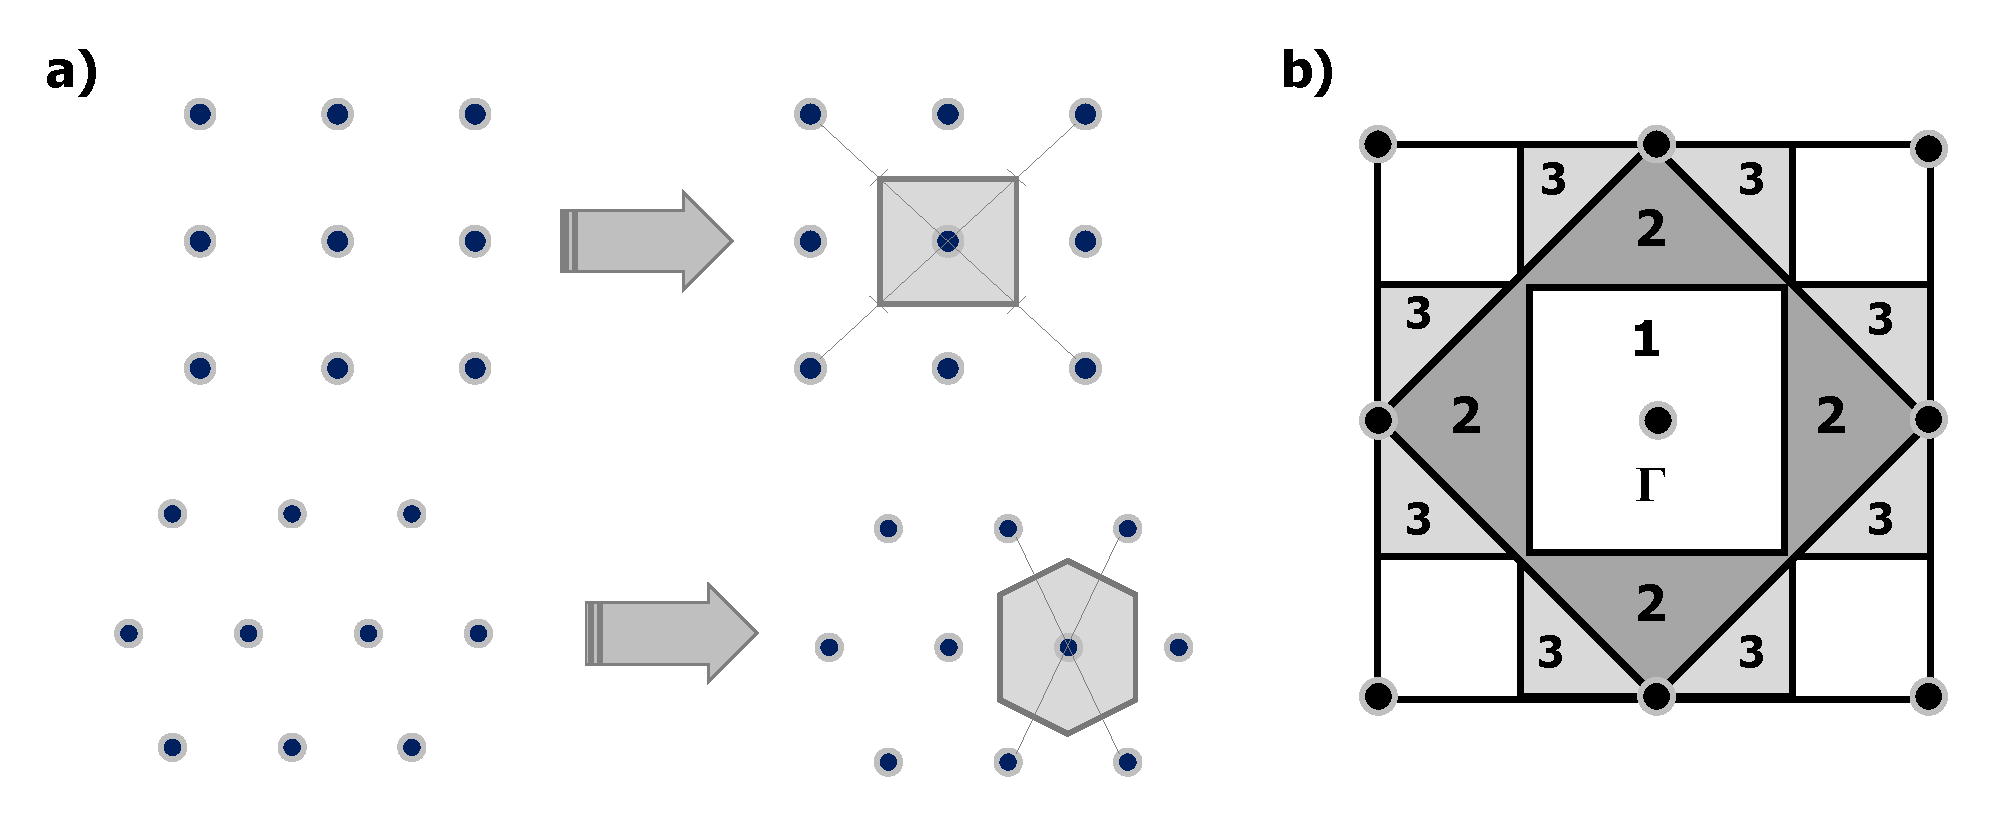
\includegraphics[scale=0.4]{capitulos/fig/intro/brillouin}
			\caption{(a) Passos para a construção da primeira zona de Brillouin (região hachurada) em uma rede bidimensional quadrada e hexagonal. (b) Representação das 3 primeiras zonas de Brillouin em uma rede quadrada no espaço recíproco.}
			\label{brillouin}
		\end{figure}

		A \textbf{primeira zona de Brillouin} é toda a região a partir da origem (conhecida como ponto $\Gamma$) que pode ser alcançada sem cruzar nenhum plano de Bragg. Existem também a segunda, terceira, ..., \textit{n}-zona de Brillouin, sendo $n-1$ o número de planos de Bragg cruzados por essa zona, como representado pela \autoref{brillouin}.
		
		Apesar de existirem diversas zonas de Brillouin possíveis, a primeira zona ocupa posição de destaque no estudo de sistemas periódicos. Como qualquer vetor de onda no espaço recíproco pode ser transladado para a primeira zona de Brillouin, toda a informação do sistema está contida nessa região do espaço recíproco. 
		
		Como o volume da célula unitária no espaço recíproco é inversamente proporcional ao volume no espaço real (\autoref{eqV}), no caso limite de uma célula de volume infinito, a primeira zona pode ser descrita somente pelo ponto $\Gamma$. Para células como volume suficientemente grande, a primeira zona de Brillouin pode ser representada por um número discreto de vetores de onda \textbf{k}. 
				
		\begin{figure}[!htb]
			\centering
			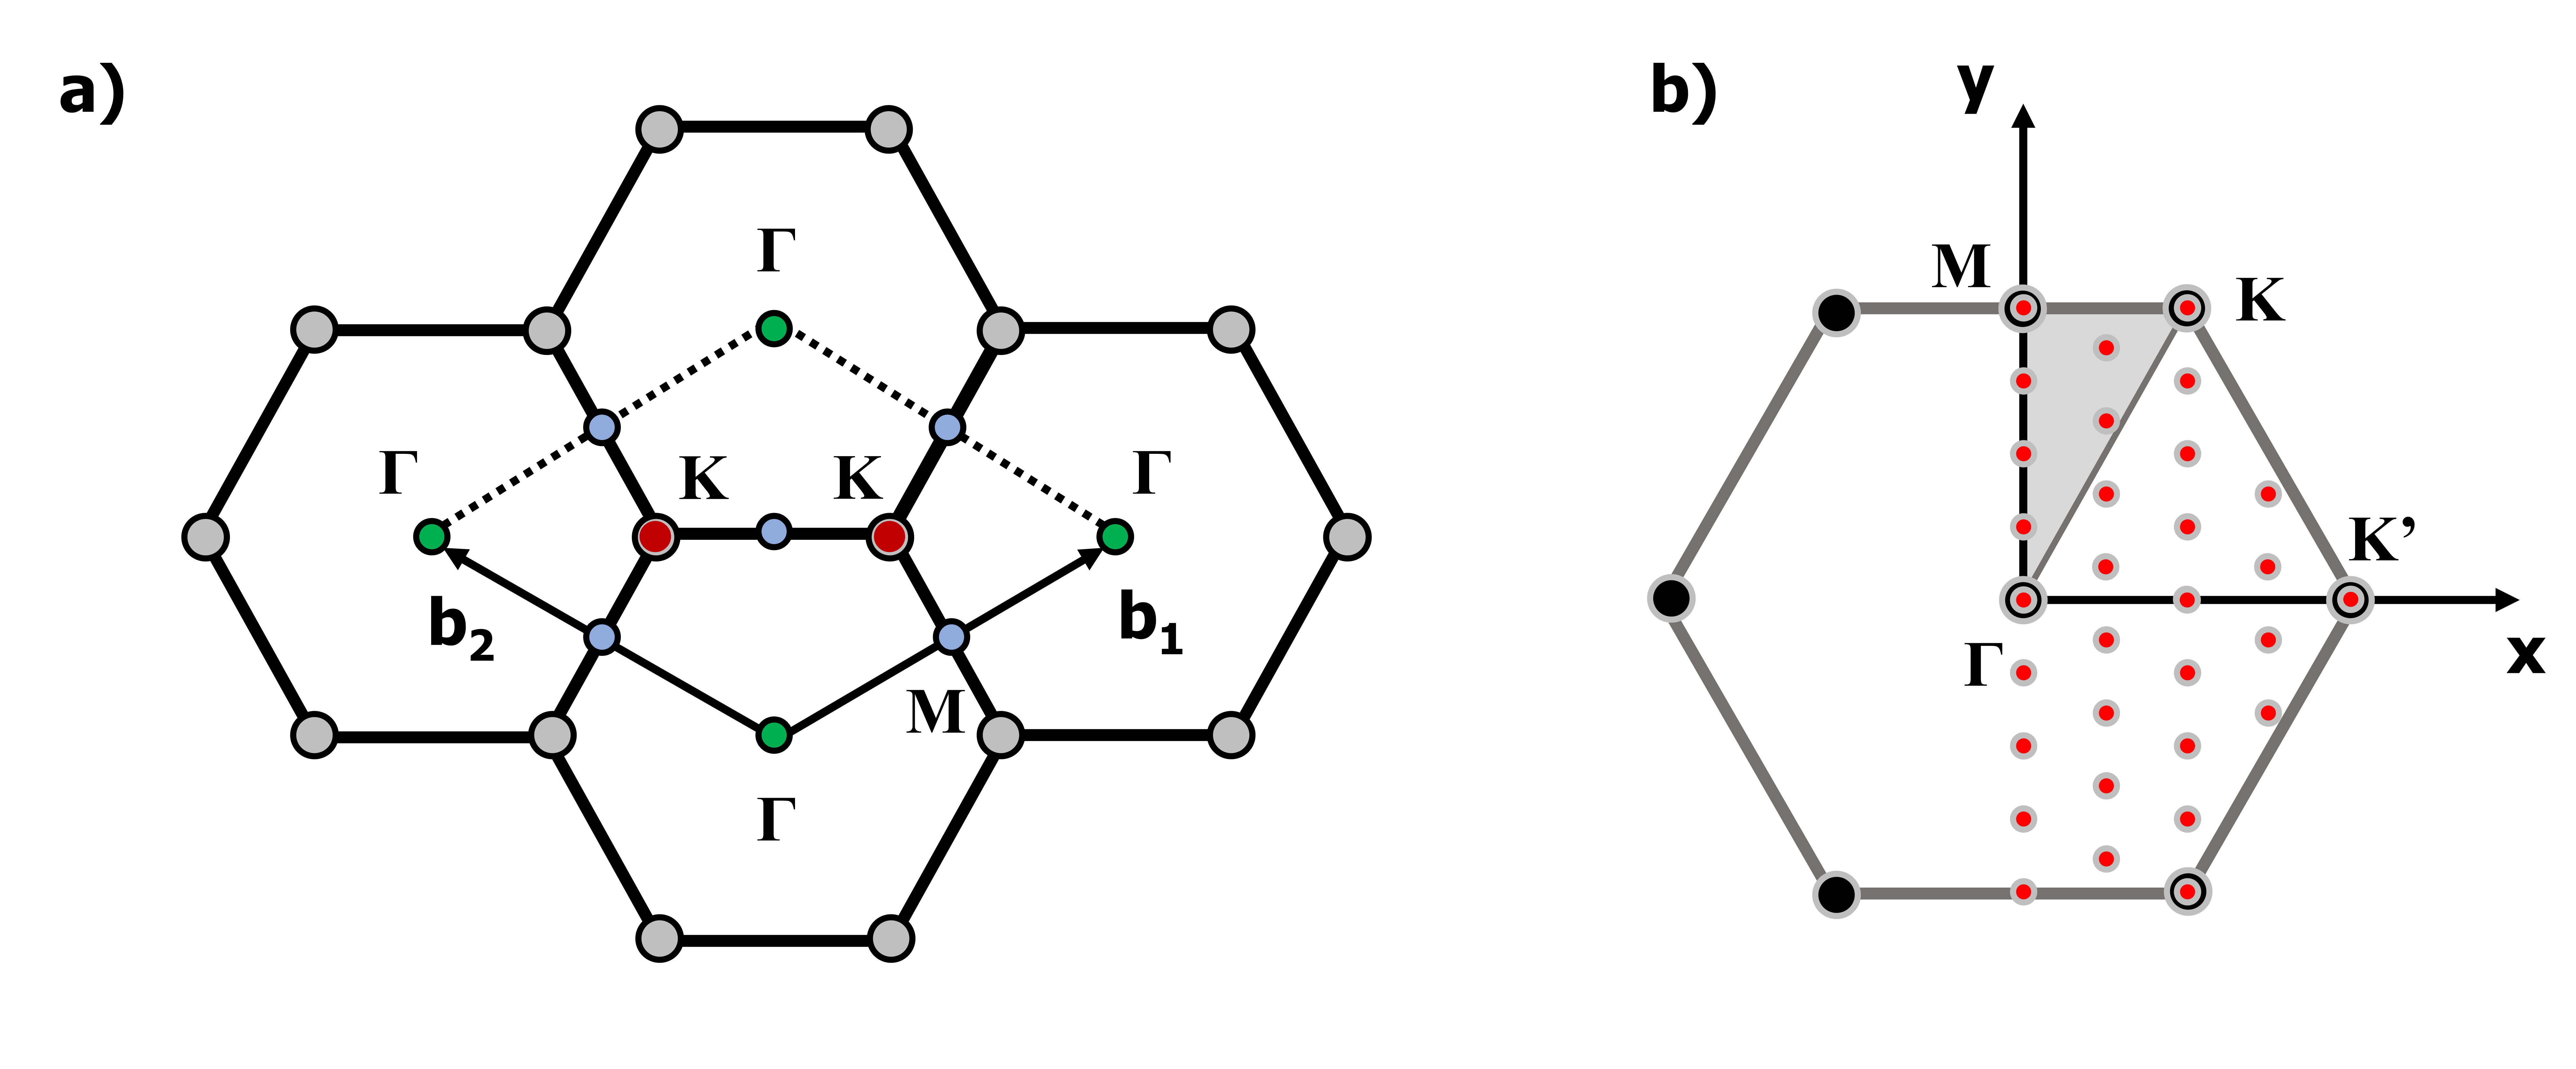
\includegraphics[scale=0.4]{capitulos/fig/intro/brillouin2}
			\caption{(a) Rede recíproca do grafeno, com a primeira zona de Brillouin definida pelos vetores $b_{1}$ e $b_{2}$ (b) Construção da zona de Brillouin irredutível e uma malha de Monkhorst-Pack de 4x4.}
			\label{brillouin2}
		\end{figure}
	
		Existem diversos métodos para gerar um conjunto de pontos satisfatórios para realizar uma amostragem do espaço recíproco. O mais utilizado é o método de Monkhorst-Pack \cite{monkhorst1976special}, onde os pontos são gerados igualmente espaçados para formar uma malha homogênea. A \autoref{brillouin2}-b) ilustra uma malha de 4x4. Quanto mais denso for a malha utilizada, melhor é o resultado e maior é a complexidade do cálculo. Em geral é feito um teste de convergência para determinar qual é a malha mínima que pode ser utilizada sem grande perda de performance. 
		
		A área hachurada \autoref{brillouin2}-b) é chamada região irredutível da primeira zona de Brillouin. Perceba que essa região quando transladada e girada consegue representar toda a primeira zona. Os pontos k que estão dentro dessa região são conhecidos como pontos não equivalentes. Como o Hamiltoniano apresenta a mesma simetria da rede de Bravais, calcular os autovalores da equação de Kohn-Sham para esses pontos é o equivalente a calcular os autovalores para todos os outros pontos. Em geral, exceto para a rede hexagonal, deslocar a malha de Monkhorst-Pack diminui o número de pontos não equivalentes, reduzindo o tempo de cálculo sem grande perda de precisão.


	\subsection{Teorema de Bloch}
	
		O teorema de Bloch afirma que as funções de onda de um elétron possuem a mesma forma de uma onda plana multiplicada por uma função que apresente a mesma periodicidade da Rede de Bravais.  Se definirmos um operador translação $\hat{T}(\mathbf{R})$ tal que $\hat{T}(\mathbf{R})f(\mathbf{r}) = f(\mathbf{r} + \mathbf{R})$, para um sistema periódico teremos
		
		\begin{equation}
			\hat{T}(\mathbf{R})\Psi(\mathbf{r}) = \Psi(\mathbf{r} + \mathbf{R}) = e^{i\mathbf{k}\cdot\mathbf{R}}\Psi(\mathbf{r}) = u_\mathbf{k}(\mathbf{r})e^{i\mathbf{k}\cdot\mathbf{R}}
		\end{equation}
		
		onde $u_k(\mathbf{r})$ apresenta a mesma periodicidade que a rede de Bravais. Dessa forma, os autoestados de qualquer operador periódico, como o Hamiltoniano, podem ser escolhidos com valores de $\mathbf{k}$ específicos que ajudam a caracterizar qualquer propriedade em um cristal periódico. 
		A função $u_k(\mathbf{r})$ pode ser expandida em uma base de ondas planas determinadas pelos vetores de onda da rede recíproca ($\mathbf{G}$) na forma
		
		\begin{equation}
			u_\mathbf{k}(\mathbf{r}) = \sum_{G=1}^{\infty} c_{\mathbf{k},\mathbf{G}}\cdot e^{i\mathbf{G}\cdot \mathbf{r}}
		\end{equation}
		
		e assim podemos escrever as funções de onda de um elétron como sendo a combinação linear de ondas planas com vetores de onda da rede recíproca, na forma
		
		\begin{equation}
		\Psi_{n,k}(\mathbf{r}) = \sum_{G=1}^{\infty} c_{n,\mathbf{k} + \mathbf{G}}\cdot e^{i\mathbf{r}\cdot (\mathbf{k} + \mathbf{G})}
		\end{equation}
		
		Do ponto de vista prático é preciso truncar esse somatório sobre os vetores $\mathbf{G}$. A forma mais usual é escolher uma energia cinética máxima de corte (E\textsubscript{cutoff}) associada a uma onda plana. Esse valor é dado por
		
		\begin{equation}
			E_{cutoff} = \frac{\hbar^2}{2m}|\mathbf{k} + \mathbf{G}|^2
		\end{equation}
		
		Para os elétrons de valência valores baixos de energia de corte conseguem ser suficientes para representar bem seu comportamento. Entretanto, para estados de caroço seria necessário um número muito grande de ondas planas para uma descrição correta. Esse problema pode ser satisfatoriamente resolvido através da utilização de pseudo-potenciais para representar os elétrons de caroço.  
	
	\subsection{Aproximação do pseudo-potencial}
	
		Essa aproximação consiste em criar uma pseudo-função de onda para representar o potencial gerado pelos elétrons de caroço na região mais próxima ao núcleo. Como nessa região os estados eletrônicos são muito localizados e suas funções de onda variam muito abruptamente, essa aproximação simplifica o cálculo permite que menos ondas planas sejam utilizadas. 

\section{Vibrações Cristalinas}

	\subsection{Cálculo das frequências de vibração}

	Como visto anteriormente, as aproximações adiabáticas e de Born-Oppenheimer permitem separar o movimento eletrônico e dos núcleos. As equações para o movimento dos elétrons são determinados pela energia total $E(\mathbf{R})$ do sistema de elétrons e núcleos, tendo a posição dos núcleos $\mathbf{R}$ como parâmetro. Se tratarmos os núcleos classicamente, a equação de movimento para cada posição nuclear $\mathbf{R}_I(t)$ fica
	
	\begin{equation}
		\label{fonon_1}
		M_I \frac{\partial^2\mathbf{R}_I}{\partial t^2} = F_I(\mathbf{R}) = -\frac{\partial}{\partial \mathbf{R}_I}E(\mathbf{R})
	\end{equation}
	
	Todos os efeitos eletrônicos estão contidos nas forças, que podem ser calculadas a partir da função de onda via teorema de Hellmann-Feynman. 
	
	Para sólidos estáveis à temperaturas moderadas, movimentos de ponto-zero, vibrações térmicas e respostas à perturbações externas podem ser descritas na forma:
	
	\begin{equation}
		C_{I, \alpha; J, \beta} = \frac{\partial^2 E(\mathbf{R})}{\partial \mathbf{R}_{I, \alpha}\partial\mathbf{R}_{J, \beta}}, C_{I, \alpha; J, \beta; K, \gamma} = \frac{\partial^3 E(\mathbf{R})}{\partial \mathbf{R}_{I, \alpha}\partial\mathbf{R}_{J, \beta} \partial\mathbf{R}_{K, \gamma}}, ...
	\end{equation}
	
	onde as letras gregas $\alpha, \beta, \gamma$ são as componentes cartesianas dos átomos $I, J, K$. 
	
	Dentro da \textit{aproximação harmônica}, os modos vibracionais de frequência $\omega$ são descritos pelos deslocamentos da posição de equilíbrio $\textbf{R}^0$
	
	\begin{equation}
		\textbf{u}_I(t) = \textbf{R}_I(t) - \textbf{R}^0_I \equiv \textbf{u}_Ie^{i\omega t}
	\end{equation}
	
	e então a \autoref{fonon_1} se torna
	
	\begin{equation}
		-\omega^2M_Iu_{I,\alpha} = -\sum_{J,\beta}C_{I, \alpha; J, \beta} u_{J,\beta}
	\end{equation}
	
	A solução completa para todos os estados vibracionais é um conjunto de osciladores independentes, cada um com frequência vibracional $\omega$, determinado pela equação clássica
	
	\begin{equation}
		det\left| \frac{1}{\sqrt{M_IM_J}}C_{I, \alpha; J, \beta} - \omega^2 \right| = 0
	\end{equation}
	
	Para cristais, os vetores de deslocamento atômico devem obedecer o teorema de Bloch, as equações da frequência vibracional são classificadas pelos vetores $\mathbf{q}$ com deslocamentos $\mathbf{u}_s(\mathbf{T_n}) \equiv \mathbf{R}_s(\mathbf{T_n}) - \mathbf{R}^0_s(\mathbf{T_n})$ dos $s$ átomos na célula caracterizada por $\mathbf{T_n}$, dado por
	
	\begin{equation}
		\mathbf{u}_{s,{\mathbf{T_n}}}= e^{i\mathbf{q}\cdot\mathbf{T_n}}\mathbf{u}_s(\mathbf{q})
	\end{equation}
	
	Combinar as duas equações anteriores permite desacoplar as equações para diferentes $\mathbf{q}$, com frequências $\omega_{i,\mathbf{q}}$, com $i=1,3s$. Essa dependência de $\mathbf{q}$ gera as chamadas \textbf{curvas de dispersão de modos vibracionais}, ou \textbf{dispersão de fônons}, que são a solução do determinante $3s x 3s$:
	
	\begin{equation}
		det\left| \frac{1}{\sqrt{M_IM_J}}C_{s, \alpha; s', \alpha'}(\mathbf{q}) - \omega_{i, \mathbf{q}}^2 \right| = 0
	\end{equation}
	
	onde a matriz reduzida das constantes de força $C$ para o vetor $\mathbf{q}$ é dada por
	
	\begin{equation}
		C_{s, \alpha; s', \alpha'}(\mathbf{q}) = \sum_{\mathbf{T_n}}e^{i\mathbf{q}\cdot\mathbf{T_n}}\mathbf{u}_s(\mathbf{q})  \frac{\partial^2 E(\mathbf{R})}{\partial \mathbf{R}_{s, \alpha}(0)\partial\mathbf{R}_{s', \alpha'}(\mathbf{T_n})} = \frac{\partial^2 E(\mathbf{R})}{\partial \mathbf{R}_{s, \alpha}(\mathbf{q})\partial\mathbf{R}_{s', \alpha'}(\mathbf{q})} 
	\end{equation}
	
	Como as vibrações são independentes, a quantização é facilmente incluída na forma usual de osciladores harmônicos: \textbf{fônons} são estados quantizados para cada oscilador com energia $\hbar \omega_{i, \mathbf{q}}$.
	
	Uma abordagem muito popular e acurada para o cálculo da matriz reduzida de constantes de força é a conhecida como \textbf{density functional perturbation theory (DFPT)}. Essa abordagem permite calcular de maneira auto-consistente a função de resposta linear à uma perturbação na função de onda e densidade de carga à uma perturbação particular para um conjunto arbitrário de vetores $\mathbf{q}$ sem a necessidade de utilização de super-células.  
	
	\subsection{Forças via teorema de Hellmann-Feynman}
		
		O teorema de Hellmann-Feynman (HF) mostra que a primeira derivada dos autovalores de um Hamiltoniano que depende de um parâmetro $\lambda$, $\hat{H_\lambda}$ é dada pelo valor esperado da derivada desse Hamiltoniano:
		
		\begin{equation}
			\frac{\partial E_\lambda}{\partial \lambda} = \left\langle \Psi_{\lambda}\left| \frac{\partial \hat{H_\lambda}}{\partial \lambda}\right|\Psi_{\lambda} \right\rangle
		\end{equation}
		
		onde $\Psi_{\lambda}$ é uma autofunção de $\hat{H_\lambda}$ que corresponde ao autovalor $E_\lambda$: $\hat{H_\lambda}\Psi_{\lambda} = E_\lambda\Psi_{\lambda}$.
		
		Na aproximação de Born-Oppenheimer, as coordenadas nucleares agem como parâmetros do Hamiltoniano eletrônico. Então, a força agindo no I-ésimo núcleo no estado eletrônico fundamental é dada por
		
		\begin{equation}
			\mathbf{F}_I = -\frac{\partial E(\mathbf{R})}{\partial \mathbf{R}_I} = -  \left\langle \Psi(\mathbf{r}, \mathbf{R})\left| \frac{\partial \hat{H}_{BO}(\mathbf{r}, \mathbf{R})}{\partial \mathbf{R}_I}\right|\Psi(\mathbf{r},\mathbf{R}) \right\rangle
		\end{equation}
		
		onde $\Psi(\mathbf{r},\mathbf{R})$ é a função de onda do estado fundamental eletrônico. Como o Hamiltoniano BO depende de $\textbf{R}$ via a interação elétron-íon, a força no átomo I é dada por
		
		\begin{equation}
			\mathbf{F}_I =- \int n_\mathbf{R}(\mathbf{r})\frac{\partial V_\mathbf{R}(\mathbf{r})}{\partial\mathbf{R}_I}d\mathbf{r} -\frac{\partial E_N(\mathbf{R})}{\partial \mathbf{R}_I} 
		\end{equation}
		
		onde $n_\mathbf{R}(\mathbf{r})$ é a densidade de carga correspondente à configuração nuclear $\mathbf{R}$ e $V_\mathbf{R}(\mathbf{r})$ é o potencial de interação elétron-núcleo
		
		\begin{equation}
			V_\mathbf{R}(\mathbf{r}) = -\sum_{i,I} \frac{Z_Ie^2}{|\mathbf{r}_i - \mathbf{R}_I|}
		\end{equation}
		
%\subsection{Dinâmica Molecular Carr-Parrinelo}
   	
\section{Quantum ESPRESSO}

	Para o desenvolvimento desse trabalho foi utilizado pacote Quantum ESPRESSO \cite{giannozzi2009quantum, giannozzi2017advanced}, que é um software livre e multi-plataforma que permite o cálculo \textit{ab-initio} de sistemas periódicos.  Este pacote é baseado na teoria do funcional da densidade (DFT) e utiliza uma base de ondas planas para expandir as funções de onda de um elétron nas equações de Khon-Sham \cite{hohenberg1964inhomogeneous, kohn1965self}. O potencial de troca e correlação será tratado utilizando a aproximação de gradiente generalizado (GGA) de Perdew-Burke-Ernzerhof (PBE) \cite{perdew1996generalized}. As interações de dispersivas foram tratadas de acordo com o modelo DFT-D3 de \citeauthoronline{grimme2010consistent} \cite{grimme2010consistent}. As interações entre os elétrons de valência com os elétrons de caroço e o núcleo foram descritas com o uso de pseudopotenciais do tipo \textit{ultrasoft} \cite{vanderbilt1990soft}. 
	
	Os parâmetros de precisão dos cálculos DFT: energia do raio de corte da energia cinética, energia do raio de corte da densidade de carga e amostragem de pontos na Zona de Brillouin segundo o critério de Monkhorst-Pack \cite{monkhorst1976special} u tiizados sao de 80 Ry, 800 Ry e 12x12x12, com base nos testes de convergência apresentados no \autoref{ap:conv}. 
	
	No processo de otimização de geometria das células unitárias será realizada a completa relaxação das posições atômicas e parâmetros de célula  até que a força total seja menor que 10\textsuperscript{-5} Ry/bohr e a variação da energia total menor que 10\textsuperscript{-4} Ry.

\section{Cálculo de Propriedades}
	
	\subsection{Equação de Estado de Murnagham}
		O módulo Bulk de um material macroscópico isotrópico é definido à temperatura constante como:
		
		\begin{equation}
			\label{bulk_def}
			B = \Omega_0\left[\frac{\partial^2u}{\partial\Omega_0}\right]_{\Omega=\Omega_0}
		\end{equation}
		
		onde $\Omega$ é o volume por átomo, $\Omega_0$ é o volume por átomo no equilíbrio e $u$ é a energia por átomo. A equação de Murnagham \cite{macdonald1969review} assume que o módulo Bulk é uma função linear da pressão, na forma:
		
		\begin{equation}
			\label{murnagham1}
			B = B_0 + PB^\prime_0
		\end{equation}
		
		Assim, para $B^\prime_0 \neq 0$, podemos escrever
		
		\begin{equation}
			\label{murnagham}
			E(V) = E_0 + B_0V_0 \left[ \frac{1}{B^\prime_0(B^\prime_0-1)}\left(\frac{V}{V_0}\right)^{1-B^\prime_0} + \frac{1}{B_0}\frac{V}{V_0} -\frac{1}{B^\prime_0 -1}\right]
		\end{equation} 
		
		O módulo Bulk foi obtido através da minimização dos mínimos quadrados, utilizando o algorítimo de Levenberg-Marquardt implementado na biblioteca SciPy \cite{jones2001scipy} para Python, nos dados de energia em função do volume para compressões hidrostáticas de $\pm$ 200 kbar.
		
	\subsection{Energia Coesiva}
		A energia coesiva, $E_c$, é definida como:
		\begin{equation}
			\label{Ec}
			E_c = E_{carbon}  - \frac{E_{tot}}{n}
		\end{equation}
		onde $E_{tot}$ é a energia total da célula unitária, $E_{carbon}$ é a energia de um átomo de carbono isolado no estado fundamental (\textsuperscript{3}P\textsubscript{0}) e $n$ é o número de átomos na célula unitária.
		
	\subsection{Deslocamento químico isotrópico}
		
		O tensor de susceptibilidade magnética foi calculado baseado na abordagem Gauge Including Projector Augmented Wave (GIPAW), implementada no código $\mathtt{gipaw.x}$ \cite{varini2013enhancement} para o Quantum ESPRESSO. A blindagem isotrópica, $\sigma_{iso}$, foi calculada para cada átomo como a média da diagonal do tensor de blindagem calculado no sistemas de eixo principal. 

		\begin{equation}
			\label{rmn}
			\sigma_{iso} = \frac{(\sigma_{xx} + \sigma_{yy} + \sigma_{zz})}{3}
		\end{equation}
		
		Os deslocamentos químicos isotrópicos ($\delta_{iso}$) foram calculados seguindo a abordagem de apresentada por \citeauthor{marques2006magnetic}, subtraindo o $\sigma_{iso}$ da blindagem isotrópica do \textsuperscript{13}C calculada para o benzeno (40.6 ppm baseado na estrutura em equilíbrio), $\sigma_{iso}^{benzene}$, e adicionado o valor do deslocamento químico isotrópico experimental do benzeno relativo ao tetrametilsilano (TMS) ($\delta^{TMS}_{benzene}$ = 126.9 ppm \cite{jameson1987gas}) para gerar o $\delta^{TMS}_{iso}$: 
		
		\begin{equation}
		\label{rmn2}
		\delta^{TMS}_{iso} = -(\sigma_{iso} - \sigma^{benzene}_{iso}) + \delta^{TMS}_{benzene}
		\end{equation}	
	
	\subsection{Dureza de Vicker}
		A dureza de Vicker de um material policristalino será calculada com base no modelo empírico desenvolvido por \citeauthor{chen2011modeling}, dado pela expressão 
		\begin{equation}
			\label{hv}
			H_v = 2(k^2G)^{0.585} - 3, \quad k = \frac{G}{B}
		\end{equation}
		
		Onde o parâmetro $k$ é chamado de módulo de Pugh e dado pela razão entre o módulo de cisalhamento ($G$) e o módulo Bulk ($B$) do material.
	
	\subsection{Função de Localização Eletrônica}
	
		O grau de deslocalização da densidade eletrônica em um sistema pode ser obtido analisando a Função de Localização Eletrônica (\textit{ELF - Electron Localization Function}). \cite{savin1992electron} Para uma única função de onda mono-determinandal construída a partir de orbitais Kohn-Sham, $\psi_i$, a ELF é definida como
		
		\begin{equation}
		\chi_{ELF} = \frac{1}{1 + (D/D_h)^2}
		\end{equation}
		
		onde 
		
		\begin{equation}
		D_h = (3/10)(3\pi^2)^{5/3}\rho^{5/3}, \quad D = (1/2)\sum_i|\nabla\psi_i|^2 - (1/8)\frac{|\nabla\rho|^2}{\rho}
		\end{equation}
		
		com $\rho \equiv \rho(\vec{r})$ sendo a densidade eletrônica. $D$ é o excesso de densidade de energia cinética local devido à repulsão de Pauli e $D_h$ é a densidade de energia cinética de Thomas-Fermi. Os valores numéricos de $\chi_{ELF}$ são convenientemente normalizados para um valor entre 0 e 1. Um valore de $\chi_{ELF}=1$ representa a localização máxima da densidade de carga, $\chi_{ELF}=0,5$ representa um gás uniforme de elétrons, \textit{i.e.} máxima deslocalização da densidade eletrônica, e  $\chi_{ELF}=0$ representa a inexistência de densidade de carga. Tipicamente, a existência de iso-superfícies com valores altos de localização da densidade eletrônica, em geral $\chi_{ELF}>0,7$, significa uma ligação localizada.   
		
	\subsection{Adsorção de gases}
		
		As simulações de adsorção de gases foram feitas utilizando Monte Carlo Grand Canonônico utilizando o software RASPA \cite{dubbeldam2016raspa}. Um potencial de Lennard-Jones foi utilizado para tratar as interações do tipo vand der Waals, com os parâmetros para as moléculas adsorvidos (N$_2$, H$_2$, CO$_2$ e O$_2$) sendo obtidos do campo de forças TraPPE \cite{potoff2001vapor} e para o adsorvente obtidas do campo de forças Universal \cite{casewit1992application}. Todas as simulações foram feitas com 10$^5$ ciclos de iniciação e 10$^5$ ciclos de produção em uma super-célula 6x6x3.
		
		
\section{Outras Informações}

	Todas as figuras do presente trabalho, exceto a \autoref{Lascaux_painting}, foram geradas pelo próprio autor utilizando a biblioteca matplotlib para Python 3 \cite{hunter2007matplotlib}, os software de visualização de estruturas VESTA \cite{momma2011vesta}, XCrysDen \cite{kokalj1999xcrysden} e Mercury \cite{macrae2006mercury} e o Microsof PowerPoint. 
